\subsection{FeSe diatomic molecule (NE-AIDMD)}
\BDB{I thought this section might fit more naturally in the examples part. I think the conclusions can discuss the shortcomings of this fit WRT fitting a lattice to a small finite system. We can also discuss moving on to superconductors in the conclusions}.
\BDB{I can put in references once we converge on the content we want to include.}

Transition metal systems are an especially difficult case for most electronic structure methods, and therefore, are an 
important test case for AIDMD. Futhermore, diffusion Monte Carlo is particularly useful in transition-metal systems, where is has been shown to improve the description of energy gaps for the types of orbital excitations used to sample the Hilbert space~\cite{lucas}.
As a test of AIDMD for transition metal systems, we consider an FeSe diatomic molecule with atomic separation 2.43 \AA~in the $z$-direction.
To our knowledge, this FeSe diatom does not exist in nature, but nevertheless serves as a simple illustration of a model for the interaction between a transition metal and ligand.
The bond distance is chosen to match the unconventional superconductor, FeSe~\cite{fese}, and therefore offer insight into a model description for that system in future calculations.

Using the process outlined in Sec.~\ref{sec:theory}, we consider a multiband Hubbard model including one iron $s$, five iron $d$ states, and three selenium $p$ states:
\begin{align*}
  H 
  &=
  \epsilon_d \sum_{i,\eta} n^{d}_{i,\eta} 
  +
  \epsilon_s \sum_{i,\eta} n^{s}_{i,\eta} 
  +
  \epsilon_\pi \sum_{i,\eta} n^{\pi}_{i,\eta} 
  +
  \epsilon_\sigma \sum_{i,\eta} n^{\sigma}_{i,\eta} 
  \\
  &+ 
  t_{\sigma} \sum_{\eta} \left( d_{z^2,\eta}^{\dagger} p_{z,\eta} + s_{\eta}^{\dagger}  p_{z,\eta} + \text{h.c.} \right)
  \\
  &+ 
  t_{\pi} \sum_{\eta} \left( d_{xy,\eta}^{\dagger} p_{x,\eta} + d_{yz,\eta}^{\dagger}  p_{y,\eta} + \text{h.c.} \right)
  \\
  &+
  U_d \sum_{i} n^{d}_{i,\uparrow} n^{d}_{i,\downarrow} 
  +
  J_d \sum_{i\ne j} S_i \cdot S_j.
\end{align*}
Here, $\eta$ represents the spin index, $\pi$ and refers to the $\pi$-bonding orbitals: $d_{xy}$, $d_{yz}$, $p_x$ and $p_y$, and $\sigma$ refers to the $\sigma$-bonding orbitals: $s$, $d_{z^2}$, and $p_z$. 
The $U_d$ interaction is between $d$ states on the iron, and the $J_d$ represents a Hunds coupling between $d$ states on the iron.
This set of parameters was chosen based on the matching pursuit method described in Sec.~\ref{sec:theory}.
%
%\BDB{This section needed?}
%The small size of the system means we can cheaply generate many samples of the space; however, this also generates an additional difficulty in generating the excited states. 
%An optical excitation in a small system will tend to shift the charge density of the system.
%As an example, the basis element formerly describing the $p_z$ state may overlap less with this new state, and to describe all the electrons in the system, one would have to use additional basis states that can describe the shift in density.
%The additional basis elements would require additional parameters, which would complicate the model. 
%To avoid this, we utilize the IAO construction \cite{IAO} of localized atomic-like basis elements for each excited state of our sample. 
%This adjusts the basis set slightly for each excited state, effectively absorbing these orbital relaxations into the definition of the basis. 
%This process can be interpreted as introducing a energy-dependence to the parameters, because basis set corresponding to the parameters now depends on the state sampled.
%As a result, we maintain a minimal Hamiltonian that describes the interaction between a single set of $s$, $p$, and $d$ orbitals, and much of the orbital relaxation effects are folded into the parameters shown above.
%

The parameters resulting from NE-AIDMD are presented in Table~\ref{tab:fese}. 
To illustrate the effect of using DMC to sample the wave functions, we also compare the results to the corresponding results from using the DFT calculations used to generate the trial wave functions. 
The states sampled consisted of singles and doubles excitations from PBE calculations with total spin 0, 2, and 4, which were then relaxed via a DMC projection.
The standard deviation of energy of the states sampled was 1.11 eV.
The $J$, $U_d$, and $t_\sigma$ were selected first by matching pursuit, as they correlated the most with the energy of the states.
A model with just these three parameters was able to achieve a root mean square error (RMSE) of 0.77 eV.
The other parameters were necessary to describe a subset of low-energy states that generally involved excitations from iron $3d$ states to iron $4s$ states. 
After adding these additional parameters, the RMSE reduced to 0.60 eV.

\BDB{Can possibly add DFT results for comparison/importance of accurate corrleation}.

The results of the parameter fit are consistent with intuition for this model. 
The $J$, $U_d$, and $t_\sigma$ are selected by matching pursuit first, and have the lowest uncertainties.
Correspondingly, the magnetic state of the iron, the interaction between $d$ electrons on the iron, and the bonding with the selenium are the most important differences between the states.
The sign of $J$ is consistent with Hund's coupling. 
The signs of $t_\sigma$ is positive, consistent with Se located in positive $z$ with respect to Fe. 
Likewise $t_\pi$ is negative corresponding to positive overlap integrals, and is smaller than $t_\sigma$ in magnitude.
The signs of each $\epsilon_i$ are describing differences in energy from exciting $d$ electrons in the iron to the 4s state.
A comparison of the model and \textit{ab initio} energies is shown in Fig. \ref{fig:fese}.
The fit is quite good considering the localized models will suffer from orbitals relaxations effects above. 

\begin{table}[ht]
\label{tab:fese}
\centering
\begin{tabular}{|c|c|}
\hline
  $\epsilon_d$       &  -0.8(2) \\
  $\epsilon_\pi$     &  0.35(8) \\
  $\epsilon_s$       &  2.4(3)  \\
  $\epsilon_\sigma$  &  -0.5(1) \\
  $t_\sigma$         &  2.6(2)  \\
  $t_\pi$            &  -0.7(2) \\
  $U_d$              &  2.9(2)  \\
  $J$                &  -0.44(4) \\
\hline
  RMSE [eV] & 0.60 \\
\hline
\end{tabular}
\caption{Downfolding parameters for FeSe diatomic molecule.}
\end{table} 

\begin{figure*}[htb]
\centering
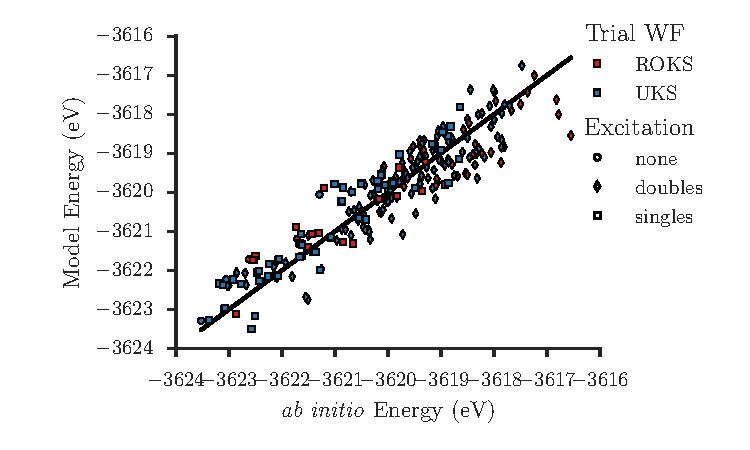
\includegraphics[width=0.7\textwidth]{./Figures/fese.pdf}
  \caption{
    Comparison of \textit{ab initio} (x-axis) and fitted energies (y-axis) of the FeSe diatomic molecule.
    \BDB{Possibly simplify this and/or add DFT results for comparison.}
  }
  \label{fig:fese}
\end{figure*}
